\documentclass[10pt]{article}
\usepackage{tikz}
\usepackage[margin=0cm]{geometry}
\pagestyle{empty}

\begin{document}

\vspace*{\fill}
\begin{center}
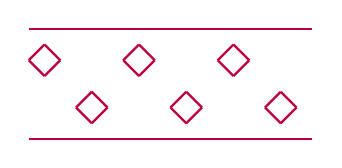
\begin{tikzpicture}[x=0.2cm, y=-0.2cm, thick, purple]
% North to South lines
% North-West to South-East lines
    \draw (1,1) -- (2,2);
    \draw (7,1) -- (8,2);
    \draw (13,1) -- (14,2);
    \draw (0,2) -- (1,3);
    \draw (6,2) -- (7,3);
    \draw (12,2) -- (13,3);
    \draw (4,4) -- (5,5);
    \draw (10,4) -- (11,5);
    \draw (16,4) -- (17,5);
    \draw (3,5) -- (4,6);
    \draw (9,5) -- (10,6);
    \draw (15,5) -- (16,6);
% West to East lines
    \draw (0,0) -- (18,0);
    \draw (0,7) -- (18,7);
% South-West to North-East lines
    \draw (0,2) -- (1,1);
    \draw (6,2) -- (7,1);
    \draw (12,2) -- (13,1);
    \draw (1,3) -- (2,2);
    \draw (7,3) -- (8,2);
    \draw (13,3) -- (14,2);
    \draw (3,5) -- (4,4);
    \draw (9,5) -- (10,4);
    \draw (15,5) -- (16,4);
    \draw (4,6) -- (5,5);
    \draw (10,6) -- (11,5);
    \draw (16,6) -- (17,5);
\end{tikzpicture}
\end{center}
\vspace*{\fill}

\end{document}
